\chapter{Gradient-Based Optimization}\label{cap:gradient}

\section{Introduction}

\section{Algorithms}

\subsection{Gradient Ascendent} 

This is the most simple algorithm to find the maximum of a function, as discussed in class (see the algorithm \ref{alg:gasc}). It is based on the idea of, starting at a random point,  iteratively improving the result by following the direction  of the gradient of the function (i.e., the derivative).

\begin{algorithm}
\SetKwData{Assign}{$\leftarrow$}
\SetKwInOut{Input}{Input}
\SetKwInOut{Output}{Output}

\caption{{\bf Gradient Ascendent\label{alg:gasc}}}
\BlankLine
\Input{Problem,$ \nabla f$, $\alpha$}
\Output{Best}
\BlankLine

\DataSty{Best} \Assign \FuncSty{RandomSolution}(Problem)

\Repeat{ found ideal solution or run out of time}
{\DataSty{Best} \Assign  \DataSty{Best} +  $\alpha \nabla$ f(\DataSty{Best})}


\KwRet{\DataSty{Best}}

\end{algorithm}

The operator $\nabla f$ computes the vector of the derivatives for each dimension. In the unidimensional case it is just $\od{f}{x}$. The way it is defined, the algorithm try to find out the \textbf{maximum} of the function. If we want the \textbf{minimum} we just have to change the add operation to a minus in the update (line 3 of the pseudo code), and we do a gradient descent algorithm. The reason why we do so is related with the sign of the derivative. In fact, if the derivative at a point is negative and we are maximizing,  the value of $x$ must be reduced, while if we are minimizing that value must be increased. The same reasoning applies when the derivative is positive (see figure \ref{fig:grad1}). 

\begin{figure}[!htbp] 
   \begin{center}
   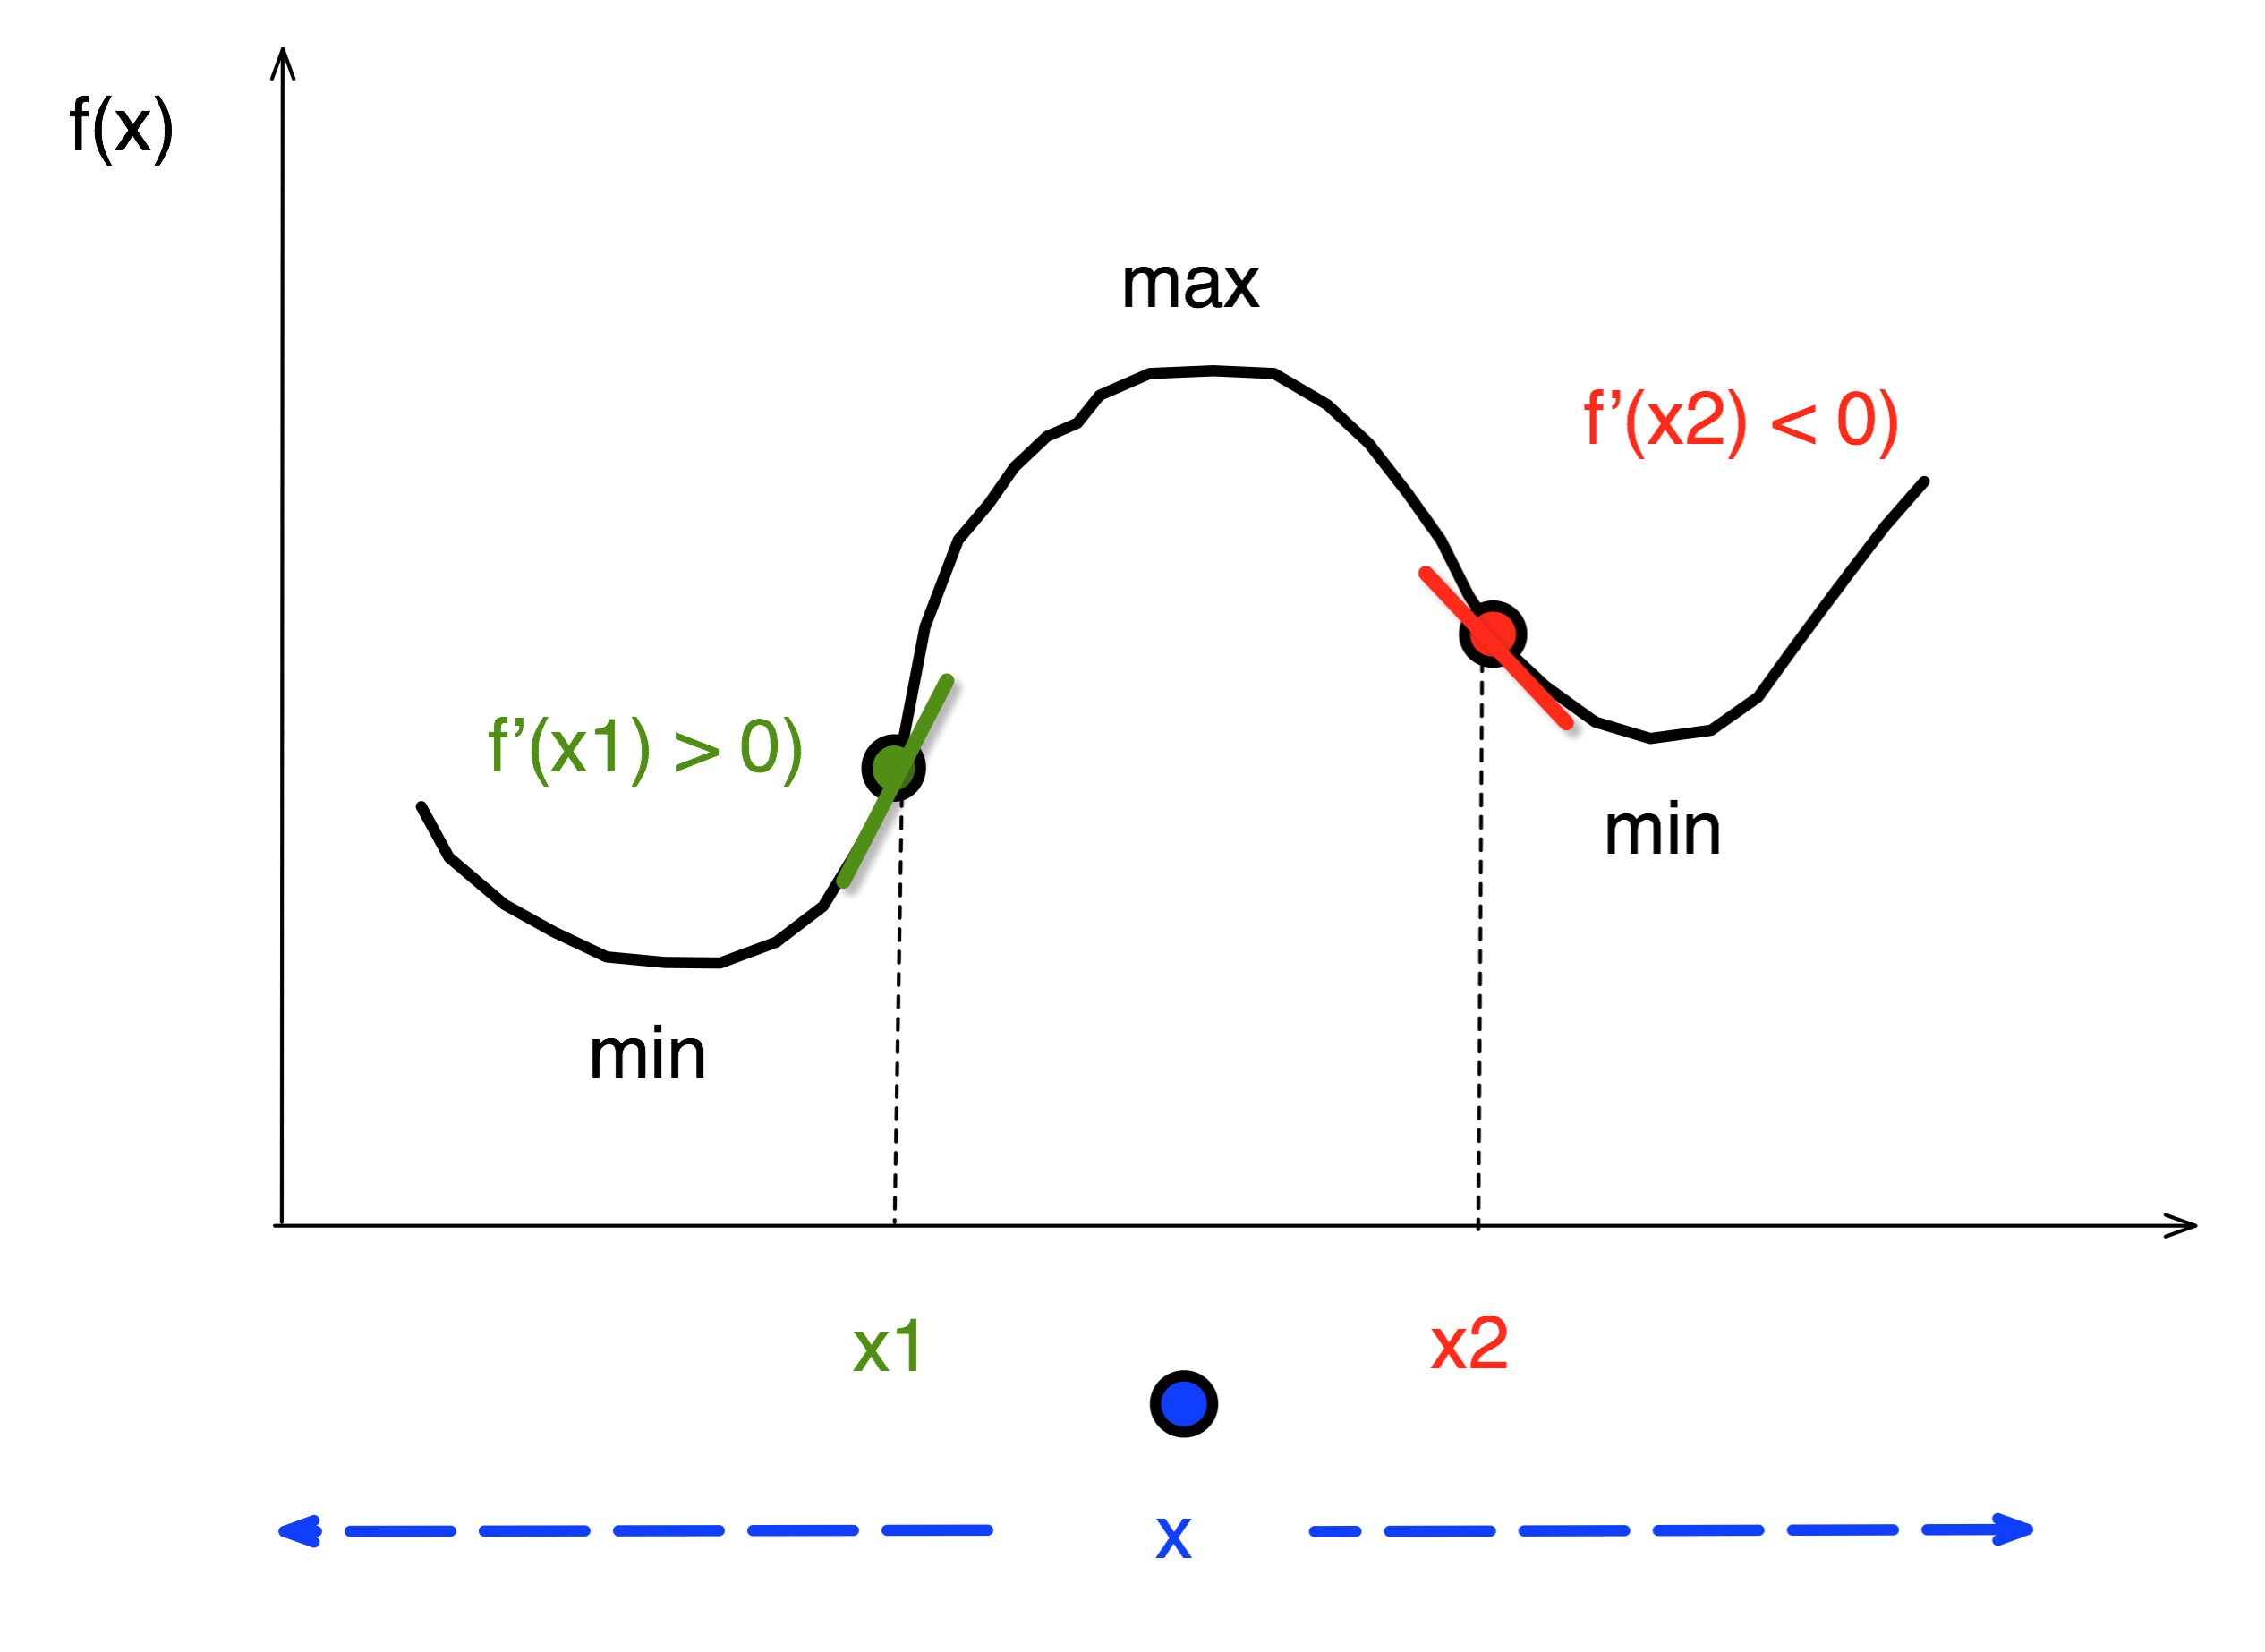
\includegraphics[scale=0.5]{cap02/imagens/grad.png} 
   \caption{When the derivative is positive (at $x_1$) the new value for $x$ must be greater if we are maximizing, smaller if we are minimizing. When the derivative is negative (at $x_2$) the new value for $x$ must be lower if we are maximizing, greater if we are minimizing.}
   \label{fig:grad1}
   \end{center}
\end{figure}



\subsection{Random Restart} 

This algorithm apply the same idea but with random restart. Algorithm \ref{alg:rnd} show the pseudo-code. As expected we now have two cycles. The external one controls how many times we perform a gradient ascendent. The idea is that trying different starting points $x$ we can avoid being trapped in a local maximum. 



\begin{algorithm}
\SetKwData{Assign}{$\leftarrow$}
\SetKwInOut{Input}{Input}
\SetKwInOut{Output}{Output}

\caption{{\bf Gradient Ascendent with random restart\label{alg:rnd}}}
\BlankLine
\Input{Problem, $f$, $ \nabla f$, $\alpha$}
\Output{Best}
\BlankLine

\DataSty{x} \Assign \FuncSty{RandomSolution}(Problem) \;
\DataSty{Best} \Assign \DataSty{x}

\Repeat{ found ideal solution or run out of time}
{
\Repeat 
	{ $|| \nabla f(\DataSty{x}) || = 0$} 
	{\DataSty{\DataSty{x}} \Assign  \DataSty{\DataSty{x}} +  $\alpha \nabla$ f(\DataSty{\DataSty{x}})}
	
\If {$f(\DataSty{x}) \ge f(\DataSty{Best})$}{ \DataSty{Best} \Assign \DataSty{x}} 

x \Assign  \FuncSty{RandomSolution}(Problem)

}

\KwRet{\DataSty{Best}}

\end{algorithm}

It should be notice here that you are not going to find a point where the derivative is \textbf{exactly} equal to zero. So you have to define an $\epsilon$ such that if $ |f'(x)| < \epsilon$ you assume the derivative is zero.


\subsection{Newton's Method}

\section{Implementation}

The implementation of these methods in Python is straightforward, in particularly for the one dimensional case.  As they are based in the idea of using the derivative (first and second) we start with a small program to compute it.  You are free to implement your own solution!

\begin{lstlisting}
def derivative(f, delta_x=0.000001):
    """Return the derivative of a function"""
    def der(x):
        return (f(x+ delta_x) - f(x)) / delta_x
    return der
\end{lstlisting}

If we want to visualize the functions, the derivatives and the evolution of the best solution over time, we also need some code.

\begin{lstlisting}
import matplotlib.pyplot as plt

def display_function(f, x_min, x_max, delta=0.1):
    x = list(frange(x_min, x_max,delta))
    y = [f(i) for i in x]
    plt.title(f.__name__)
    plt.grid(True)
    plt.axhline(c='black')
    plt.axvline(c='black')    
    plt.xlabel('X')
    plt.ylabel('Y= '+f.__name__ + '(X)')
    plt.plot(x,y, 'r')
    plt.show()
\end{lstlisting}

\paragraph{frange}Notice the use of a function (\texttt{frange}, equivalent to  \texttt{range} but that works with floats. As there is not such a thing in Python\footnote{If you are using Python arrays this is not true, for we have the \texttt{arange} method in the \texttt{numpy} module.}, let's implement it too.

\begin{lstlisting}
def frange(n1,n2=None,n3=1.0):
    """
    Range with floats.
    Can be called as  with range:
    frange(n)
    frange(n1,n2)
    fange(n1,n2,n3)
    """
    if n2 == None:
        n2 = n1
        n1 = 0.0
    nextn = n1
    while (n3 >= 0.0 and nextn <= n2) or (n3 < 0.0 and nextn >= n2):
        yield nextn
        nextn += n3
\end{lstlisting}


-- INCLUDE: code for the evolution of the best solution...\\


\section{Exercices}